\chapter{Detection and Characterisation of rotational spherical aggregate rotational dynamics}
\label{chapter:simulated_detection}
As outlined in the end of Chapter 4, one of the difficulties 
in characterising interactions with asymmetric objects is 
the coupled motion between translation and rotation. In order
to characterise the optical trap a position detection system 
such as a lateral effect photodiode or a quadrant photo diode
(see fig.\ref{fig:position_detectors}). Typically, a position 
detection system assumes that there exists a linear relationship 
between the a particle's displacement and the detected signal.
However, this is not always the case as demonstrated in chapter
4; as dimer's demonstrate non-harmonic trapping beyond a certain 
displacement. In addition, the rotational effects of the trapped
dimer become a more significant factor when characterising the 
trap strength. This can have unintended effects when it comes to
areas of research that require a precise understanding of the 
hydrodynamic behaviour of particles. As such there has been a 
concerted effort to either eliminate rotational motion, or describe
how the rotational behaviour influences the trajectory reported 
by the position detector. 

Rotational motion about a single axis is easiest to account for.  
When the power spectra of elliptical polystyrene particles was 
fitted by Yogesh \textit{et al} \cite{Yogesha2011PreciseCO}, they 
assumed that the rotational motion was purely in the transverse
plane. As such they did not have to account for any variance in 
the trapping strength due to orientation nor did they need to
consider non-periodic rotational behaviour. In the case where 
rotational motion is stochastic the problem is more complex. 
For example, when an optical fibre trap characterisation 
technique was implemented by Saffron \textit{et al} 
\cite{BarZiv1997, Meller1998}, they were able to use dynamic 
light scattering to characterise both the axial and lateral 
trap stiffness acting on microspheres. The only drawback 
admitted to in their work was that the technique was constrained 
to isotropic scatters as their theoretical model for describing 
the auto-correlation function was predicated on the fact that 
any variations in the signal are due to the particles 
translational motion within the confines of a cylindrical trap 
\cite{BarZiv1997}. Where the upper limit of the cylindrical 
trap is given by the Rayleigh range ($z_R = n\omega_0/NA$).
However, as demonstrated by the results from Chapter 4.1, 
the axial traps of spherical aggregates is often situated 
far beyond the Rayleigh range (for a 1.2 NA laser this is 
$\pm5.985 \mu m$).

To accurately describe the full dynamics of an anisotropic
scatterer its clear that additional characterisation 
techniques are necessary. In this chapter we demonstrate 
two such techniques, quadrant photo-diode simulation, and 
an optical fibre static light scattering arrangement. The 
former is based on the work of Rohrbach and Stelzer 
\cite{Rohrbach2002}, where their work is limited to single 
spheres, we extend the possible particle space to allow for 
any theoretical combination of spheres. The results from
chapter 4 demonstrate that the rotational motion causes 
significant deviations between the computed trapping strength
and the expected trapping strength according to Lorenz-Mie
theory. By utilizing vector regression we can accurately 
recreate a particle's trajectory simply from the QPD signal, 
both in the transverse plane and along the beam axis. 

The latter method builds upon \cite{BarZiv1997} but now 
accounts for the full rotational motion. This was initially
developed in tandem with the work conducted in chapter 3,
with the idea being that if a crystal nucleus formed on a 
rotating sphere how would that nucleus influence the motion
of the rotating sphere. Using static light scattering we can 
map the outputted signal from a optically trapped dimer to 
its expected orientation in real time. Thus allowing us to 
estimate the optical torque being applied to the dimer by 
the trapping beam. As demonstrated in chapter 4, the 
influence of a circularly polarised beam can result in 
gyroscopic precession for specifically sized dimers. 

We start by outlining the working principle behind the
optical fibre detection system, before demonstrating 
how it can be used to instantaneously predict 
orientational information on a trapped particle. We then
consider common factors of error in the characterisation
process, such as signal error, and incorrect particle 
sizing. Both of which have a significant impact on the 
performance of the model, but by utilising Bayesian 
inference, and time averaging we can better refine our 
model.   

\section{Monitoring Stochastic rotational motion using static 
		light scattering}
Part of the optical fibre arrangement borrows code from the 
optical tweezer simulations discussed in Chapter 2 and 4. 
Rather than repeat the simulation details we will instead 
only focus on the specifics of the optical fibre scattering.

\subsection{Coordinate System}
Consider a particle (either a sphere or dimer) trapped by
a Gaussian beam, with its focal point being set at [0,0,0]. 
At the same time an optical fibre directs a plane wave that 
is incident on the trapped particle scattering light in all 
directions. The probe beam is assumed to be x-polarised and 
propagating in the +z direction, this is a $90^{\circ}$ 
rotation from the previous simulations (see fig\emph{X.X}). 

\subsection{Dimer}
The dimer is defined by two spheres with refractive indices
of 1.59 and suspended in water ($n_{med} = 1.33$). \textit{MSTM}
requires a target origin for setting the scattering expansion, as
with our simulations we set it as the dimer's centre of diffusion.
The near field scattering from the dimer is shown in 
fig.~\ref{fig:nf_scattering}.

\begin{figure}[h!]
	\centering
	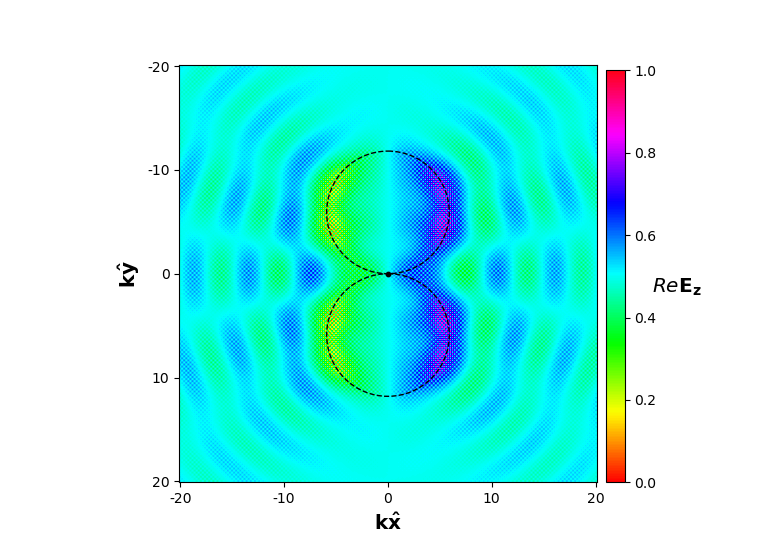
\includegraphics[width=\linewidth]{nf_scattering_dimer.png}
	\caption{Re ${\bf E_z}$ distribution from a symmetric dimer when 
	irradiated by the probe beam (viewed in the x-y plane). Axis are 
	given in dimensionless units of $k\hat{x}$ and $k\hat{y}$ respectively.}
	\label{fig:nf_scattering}
\end{figure}

\subsection{Detectors and Pixels}
Each detector is placed some distance $\bf r$ from the origin, 
detector positions are defined by angles $\theta$ \& $\phi$. With 
$\theta=\phi=0$ being directly in front of the probe beam. The 
position of each detector is given by:
\begin{align}
	[x_{fiber}, y_{fiber}, z_{fiber}] = [rcos(\phi)sin(\theta), rsin(\phi)sin(\theta), rcos(\theta)]
\end{align}
Where r is the distance between the detector and the target origin. 
In an ideal situation the surface of the detector is oriented towards 
the target origin perfectly. Pixels can be thought of as points lying 
on the surface of the detector, each point has its own position in real
space. Using \textit{mstm} we can find the components of the scattering 
matrix at each point and compute the intensity of the electric field via:

\begin{align}
	\begin{pmatrix}
		I_s \\ Q_s \\ U_s \\ V_s
	\end{pmatrix} = 
	\begin{pmatrix}
		S_{11} & S_{12} & S_{13} & S_{14} \\
		S_{21} & S_{22} & S_{23} & S_{24} \\
		S_{31} & S_{32} & S_{33} & S_{34} \\
		S_{41} & S_{42} & S_{43} & S_{44} \\
	\end{pmatrix}
	\begin{pmatrix}
		I_i \\ Q_i \\ U_i \\ V_i
	\end{pmatrix}
\end{align}
Where:
\begin{align}
	I_s &= E_{x,\ scat}^2+E_{y,\ scat}^2 \\
	\rightarrow I_s &= S_{11}I_i+S_{12}Q_i+S_{13}U_i+S_{14}V_i
\end{align}

By computing the scattering at each point on the detectors surface 
we can compute the average scattering over the detector. As the 
detectors are moved further away from the target origin the intensity 
distribution across the detector surface falls off until near uniform.


By moving the detectors further back we can treat each detector as single
point and compute the intensity at the centre of the detector rather than
consider the full surface.

\section{Interpretation of scattering data into orientation estimates}
Consider a dimer in the optical trap (Fig.~\ref{fig:dimer}a), we can define at any 
point in time a unit vector $\hat{s}$ pointing from the centre of the larger sphere 
to the centre of the smaller sphere. A plane wave probe beam is incident on 
the trapping laser, is incident on the dimer, generating a scattering pattern
dependent on the dimer's orientation $I(\hat{\bf s}, \theta, \phi)$ which can be 
computed using \textit{mstm} \cite{I.Mishchenko1996}. To represent the experimental 
set up consisting of a set of optical fibres recording scattered light, we choose 
four sets of spherical angles [$(\theta_1,\ \phi_1), \ (\theta_2,\ \phi_2), \ 
(\theta_3, \ \phi_3), \ (\theta_4,\ \phi_4)$] and record the calculated intensity 
at each angle $I(\hat{s},\ \theta_k,\ \phi_k)$. 

\begin{figure}[h!]
	\centering
	\begin{subfigure}{0.49\textwidth}
		\subcaption{}
		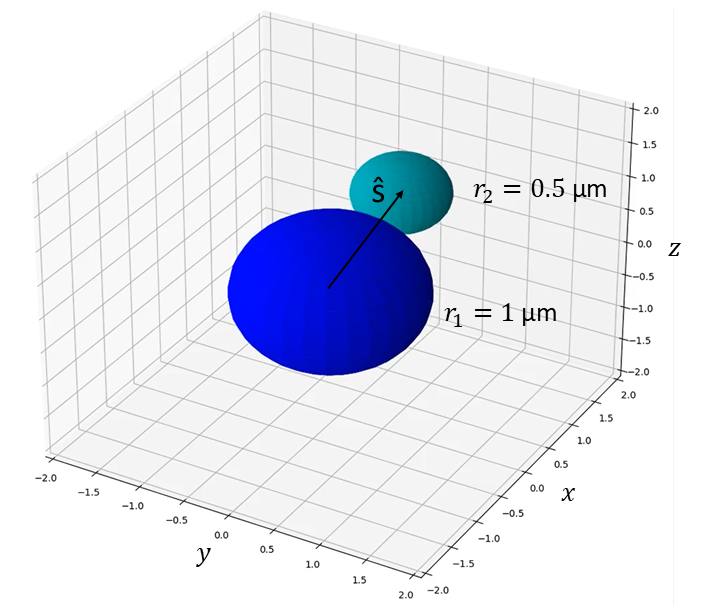
\includegraphics[width=\textwidth]{fig2a.png}
	\end{subfigure}
	\begin{subfigure}{0.49\textwidth}
		\subcaption{}
		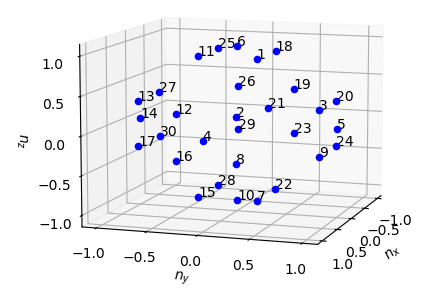
\includegraphics[width=\textwidth]{fig2b.png}
	\end{subfigure}
	\caption{(a)Example dimer in orientation $\hat{\bf s}$, (b) 30 Reference orientations represented by vectors pointing from [0,0,0] to each point}
	\label{fig:dimer}
\end{figure}

Our goal is to determine the orientation of the trapped dimer based on the measured 
intensity $I(\hat{n}, \ \theta_k)$. Rather than aim immediately for an exact estimate 
of the dimer's orientation, for the purposes of interpretation of the scattering and 
optimisation of the measurement setup it is more convenient to discretize the possible orientation space into a number of possible reference orientations, which we can then 
use as 'classification categories' in a neural network methodology to map scattering 
data to orientation (see below for further discussion).  Here we choose $\textit{n}_{ref} 
\ = \ 30$ reference orientations $\hat{\bf n}_{\alpha}$  evenly distributed on a 
unit sphere \cite{Reyuthor2006} (Figure~\ref{fig:dimer}b) leading to a maximum 
nearest-neighbour spacing between two neighbouring reference orientations of 0.895 
radians. Using MSTM we compute the raw intensities at each of the measurement angles 
that would be generated by a dimer in each reference orientation, $I(\hat{\bf n}_{\alpha}, \theta_k)$. While the number and position of detection fibres is technically arbitrary 
there are several constraining factors that limit our ability to infer useful information 
from the trapped object, see Section~\ref{sec:detectors} for a detailed breakdown 
of our choice of detection angles. The raw intensities are normalized according to:
\begin{align}
	\label{eq:scale}
	y_k(\hat{\bf n}_\alpha)
	= 
	\frac{I(\hat{\bf n}_\alpha, \theta_k) - \langle I(\hat{\bf n},\theta_k) \rangle } 
	{\langle I^2(\hat{\bf n},\theta_k) \rangle -\langle I(\hat{\bf n}, \theta_k)\rangle^2}
\end{align}

where the denominator is simply the standard deviation across the set of values
$I(\hat{\bf n}, \theta_k)$. The reference orientations, raw intensities, and scaled 
signals are given in Tables~\ref{tab:A1} and \ref{tab:A2}. 

Note that the collected scattering signals are not necessarily simply related to 
their associated reference orientations: as is well known from such examples of 
the inverse scattering problem. While it is trivial to compute the light scattering 
pattern for any given particle with any particular characteristic (i.e. size, 
shape, or orientation), inferring the light scattering from a unknown particle 
to determine said characteristic is incredibly difficult due to complex mapping 
between scattering and said characteristic. Even if the orientation space is divided 
evenly between reference orientation the subsequent signal space ends up being 
appearing mixed making simple comparisons of signals useless for inferring information 
on the particle. Shown below is two clusters of orientation vectors and there 
respective measured scattering signals - the points have been coloured based on 
their proximity to the centre of their respective cluster. While the orientation 
space appears tightly packed and ordered the signal space quickly spreads out in 
an asymmetric fashion. Furthermore as seen in Fig~\ref{fig:mixing}b the signal 
mapping can intersect itself which only further increases the complexity. While 
in some instances the mapping between one reference orientation and another is 
discrete, in other instances the mapping becomes far more complex to discern. 

\begin{figure}[h!]
	\centering
	\begin{subfigure}{0.4\textwidth}
		\subcaption{}
		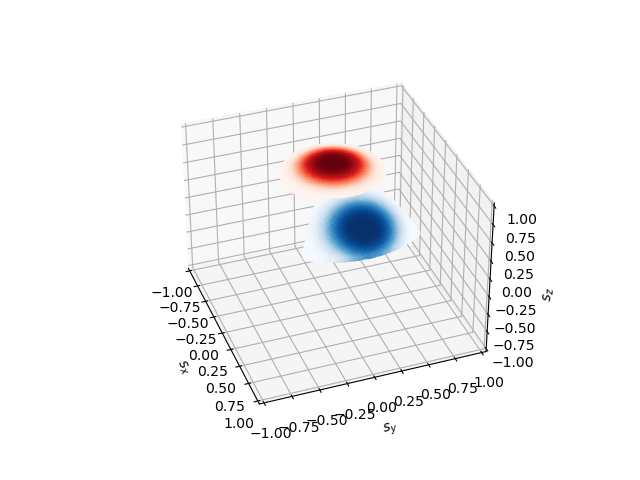
\includegraphics[width=\textwidth]{fig3a.png}
	\end{subfigure}
	\begin{subfigure}{0.4\textwidth}
		\subcaption{}
		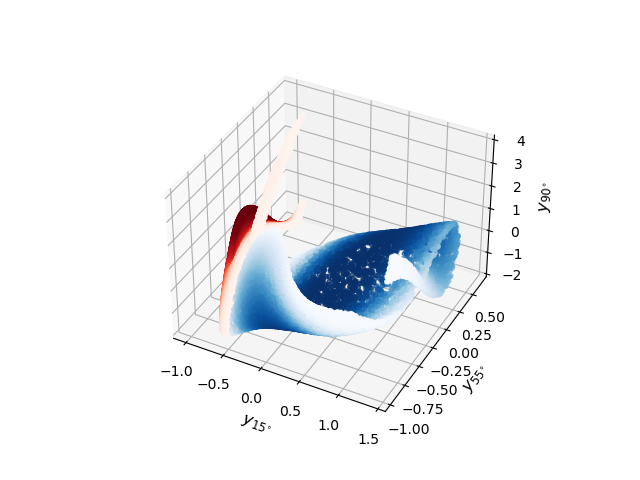
\includegraphics[width=\textwidth]{fig3b.png}
	\end{subfigure}
	\caption{(a) Distribution of orientation vectors and (b) their respective scattering signals. Points are coloured according to their distance from the centre of each cluster (red points centred around [$0.00, 0.00, 1.00$], blue points centred at [$0.71, 0.00, 0.71$])}
	\label{fig:mixing}
\end{figure}

Nevertheless, at least where the uncertainty in signal measurements is low (see 
below), we can predict the orientation from the scattering by utilising 
computational techniques such as neural networks. We thus utilised the Python 
machine learning program \textit{scikit-learn} \cite{Pedregosa2011} to build a 
neural network for identifying the dimer's orientation from its light scattering 
signal. The network was trained by generating a database of random orientation 
vectors, calculating the corresponding light scattering signals, and then using 
the network to estimate the probability of a given signal coming from a dimer in 
a given reference orientation. The network's loss function was evaluated and used 
to improve the estimation, the network being trained until the improvement in the 
loss function was less than 0.0001. 

Importantly, the estimation provided by the neural network can be improved further 
by accounting for any prior information we know about the dimer, utilising Bayesian 
inference to update the neural network's estimation: 
\begin{align}
	\label{eq:bayes}
	p(\hat{\bf n}_\alpha| y_k(\hat{\bf s}))
	&=
	\frac{p(y_k(\hat{\bf s})|\hat{\bf n}_\alpha)
		p(\hat{\bf n}_\alpha)}{p(y_k(\hat{\bf s}))}
\end{align}

where $p(\hat{\bf n}_\alpha)$ and $p(y_1, y_2, y_3)$ are the prior estimates of 
the distributions of particle orientations and instantaneous signals, respectively.
\textit{Without} any prior evidence we must assume that the orientation prior of 
the dimer $p(\hat{\bf n}_{\alpha})$ is uniform. However, inference about the 
dimer's possible current orientation from knowledge of previous measurements can 
be used to inform our estimate of $p(\hat{\bf n}_{\alpha})$. The latter prior 
$p(y)$ is the probability of measuring a signal ($y_1$, $y_2$, $y_3$). This is 
given by taking the discrete integral over the collection of reference orientations:
\begin{align}
	p(y_1, y_2, y_3, y_4)
	=
	\sum_{\alpha=1}^{n_{\rm ref}}
	p(y_1, y_2, y_3, y_4|\hat{\bf n}_\alpha)
	p(\hat{\bf n}_\alpha)
\end{align}

From \eqref{eq:bayes} we obtain the key result, a mass probability distribution 
denoting the probability that our dimer is in orientation $\hat{\bf n}_{\alpha}$ 
given a measured signal ($y_1$, $y_2$, $y_3$), \textit{i.e.} an estimated mapping 
from scattering measurement to orientation estimate. 

%%%%%%%%%%%%%%%%%%%%%%%%%%%%%%%%%%%%%%%%%%%%%%%%%%%%%%%%%%%%%%%%%%%%%
\subsection{Calculation of error}
\label{sec:divergence}
To evaluate the above estimation of dimer orientation from scattering signal, we use a Brownian simulation of a dimer in the optical trap (Section~\ref{sec:brownian}) to compare estimated most probable reference orientation, derived from the dimer's scattering through Eq.~\eqref{eq:bayes}, with the dimer's known \emph{actual} orientation $\hat{\bf s}$. MSTM provides calculated light scattering from the simulated dimer $I(\hat{\bf s}, \theta)$ and we use \eqref{eq:scale} to obtain normalized values at each measurement angle $\theta_k$,  $y_1(\hat{\bf s})$, $y_2(\hat{\bf s})$, $y_3(\hat{\bf s})$, from which we obtain $p(\hat{\bf n}_{\alpha}\parallel y_1, y_2, y_3)$. Because we know the actual orientation $\hat{s}$ we can measure the error in the model's estimate by comparing the reference orientation closest to $\hat{s}$, denoted as $\hat{\bf n}_{best}$, with the most probable predicted orientation from Eq.~\eqref{eq:bayes}. An ideal result would be one where the probability distribution is 0 for every $\hat{\bf n}$ apart from $\hat{\bf n}_{best}$:
\begin{align}
	\label{eq:best}
	p_{best} = 
	\begin{cases}
		1 & \text{when $\hat{\bf n}_\alpha$ = $\hat{\bf n}_{best}$}\\
		0 & \text{anywhere else}
	\end{cases}
\end{align}
In reality the distribution from Eq.~\eqref{eq:bayes} will assign some non-zero
probability to every reference orientation, leading to some level 'confidence' in orientation prediction, which can be quantified by calculating the Kullback-Leibler divergence $K_l$ between the two distributions:
\begin{align}
	K_{l, \#}(p_{best}\parallel p(\hat{\bf n}_\alpha| y_1, y_2, y_3))
	= p_{best}\ln \left[\frac{p_{best}}{p(\hat{\bf n}_{best}| y_1,y_2,y_3))}
	\right]
	\label{eq;kullback}
\end{align}
where a larger value of $K_l$ indicates that our model is less confident in its
prediction of the dimer's orientation. The divergence $K_l$ thus illustrates the 'spread'
in the estimated dimer orientation probability --- a distribution strongly peaked at 
some value would give us more confidence in that value than a near-uniform distribution 
where the scattering measurement could imply a wide range of possible orientations --- 
but it does not directly indicate our estimates actual accuracy, that can be simply defined as the percentage of our estimations that are correct. 

%%%%%%%%%%%%%%%%%%%%%%%%%%%%%%%%%%%%%%%%%%%%%%%%%%%%%%%%%%%%%%%%%%%%%
%%%%%%%%%%%%%%%%%%%%%%%%%%%%%%%%%%%%%%%%%%%%%%%%%%%%%%%%%%%%%%%%%%%%%
\subsection{Brownian Simulation}
\label{sec:brownian}

We use the Brownian OT package developed by Fung~\textit{et~al} \cite{Vigilante2020Brownian_OT} to simulate the motion of an asymmetric dimer (Figure~\ref{fig:dimer}a) within an optical trap. Brownian OT combines MSTM \cite{Mishchenko1996MSTM} and ``Optical Tweezer Toolbox'' (\textit{ott}) \cite{Lenton2020} to simulate the motion of arbitrary
shaped sphere clusters. We simulate the motion of a dimer trapped in a highly focused Gaussian beam by calculating the optical forces imparted by the laser, and the Brownian force due to the surrounding fluid. MSTM provides the necessary T-matrix to compute the optical force via \textit{ott}. The Brownian force is found by computing the dimer's diffusion tensor according to the analytical solutions provided by Nir and Acrivos \cite{nir_acrivos_1973}. We simulated a polystyrene dimer ($n = 1.59$) in a suspension of water ($n_{med} = 1.33$) over the course of $1 \ s$ with a simulation time step of $1 \times 10^{-5} \ s$. We placed the dimer 4 microns below the trap focus at an angle $30^{\circ}$ from the horizontal, the resulting trajectory is shown below in Sec~\ref{sec:motion}. We chose these initial parameters because it demonstrates our model's performance in non steady state conditions. 

The exact number of detectors was initially assumed to be arbitrary, in that it made no difference to our estimate whether we used 2 angles or 200. For practical purposes it seemed beneficial that we demonstrate our method works for a minimal number of detection angles, as geometric constraints come into play when trying to install a high number of detection fibres for any optical tweezer set up. 


\begin{figure}[h!]
	\centering
	\begin{subfigure}{0.49\textwidth}
		\subcaption{}
		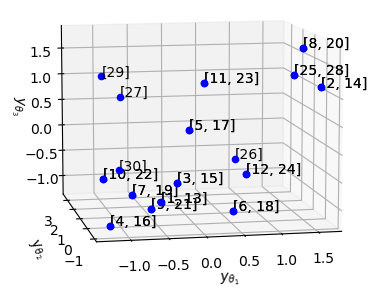
\includegraphics[width=\textwidth]{fig4a.png}
	\end{subfigure}
	\begin{subfigure}{0.4\textwidth}
		\subcaption{}
		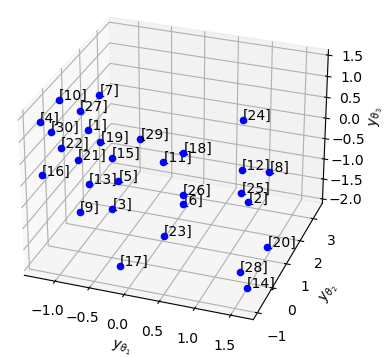
\includegraphics[width=\textwidth]{fig4b.png}
	\end{subfigure}
	\caption{Expected scattered signals from reference orientations -see fig~\ref{fig:dimer} - when: (a) all three detectors are in the X-Y plane, (b) when 1 detector is raised out of the X-Y plane.}
	\label{fig:detectors}
\end{figure}

When all of the detectors lie in the same plane the expected signal can appear identical despite the dimer being in completely different orientations. This is shown in Figure~\ref{fig:detectors} which plots the expected signals from 30 reference orientations, each point is labelled with its corresponding reference orientation, the fact that points have multiple labels is because the dimer's scattering is indistinguishable in these two reference orientation. It should be noted that these pairs are reflected in one or more axis which suggests that these are due to the arrangement of our detectors. More specifically, if the detectors are placed say in the x-y plane then only when the dimer is pointed nearly fully upright will the expected signal be entirely unique. This is illustrative of the difficulty behind the inverse light scattering problem; as one cannot always map a given signal to a particular parameter value.

To remedy this we raise the third detector out of the x-y plane; as such the expected signals from each reference orientation is unique. As seen between Figures \ref{fig:detectors}a \& b each reference orientation now has a unique scattering signal, though with only three detectors the difference in expected signals can appear insignificant. By adding a $4^{th}$ detector we can differentiate signals more reliably, improving the neural networks performance.   In line with our goal of making this method viable in a laboratory setting we decided not to increase the number of detectors further than 4. 

%%%%%%%%%%%%%%%%%%%%%%%%%%%%%%%%%%%%%%%%%%%%%%%%%%%%%%%%%%%%%%%%%%%%%
\subsection{Testing the Model}
\label{sec:test}
Using our simulation from Section~\ref{sec:brownian} we simulated the motion of a silica dimer ($n = 1.45$) trapped in water ($n = 1.33$) within a 5 mW optical trap. The trapping laser is 1064nm NIR focused through a 1.25 NA objective. The dimer is comprised of two tangent spheres with radii $1 \mu m$ and $0.5 \mu m$ respectively. We simulated the first 10 seconds of motion, calculating the orientation and position every 1 ms. 

We applied Eq.~\eqref{eq:bayes}, taking the reference orientation with the highest probability  as our estimate of the dimer's instantaneous orientation $\hat{\bf n}_{est}$. To visualise the model's performance  we plotted the radial distance between our estimation $\hat{\bf n}_{est}$ and the dimer's \emph{actual} instantaneous orientation $\hat{\bf s}$ versus time. For comparison, we also plotted the radian distance between the  dimer's instantaneous orientation and the closest reference orientation, denoted $\hat{\bf n}_{best}$. The dotted line indicates the maximum radian distance ($0.896$ radians) between two \textit{neighbouring} reference orientations: if we are under this line then we know our estimate is at least neighbouring the best result. Assuming a uniform prior of the reference orientations $p(\hat{\bf n}_\alpha)$  the neural network's predictions ($\hat{\bf n}_{est}$ from Eq.~\eqref{eq:bayes}) are at times reasonable, but there are significant large and random jumps away from the correct result (Fig.~\ref{fig:uniform}). 

\begin{figure}[h!]
	\centering
	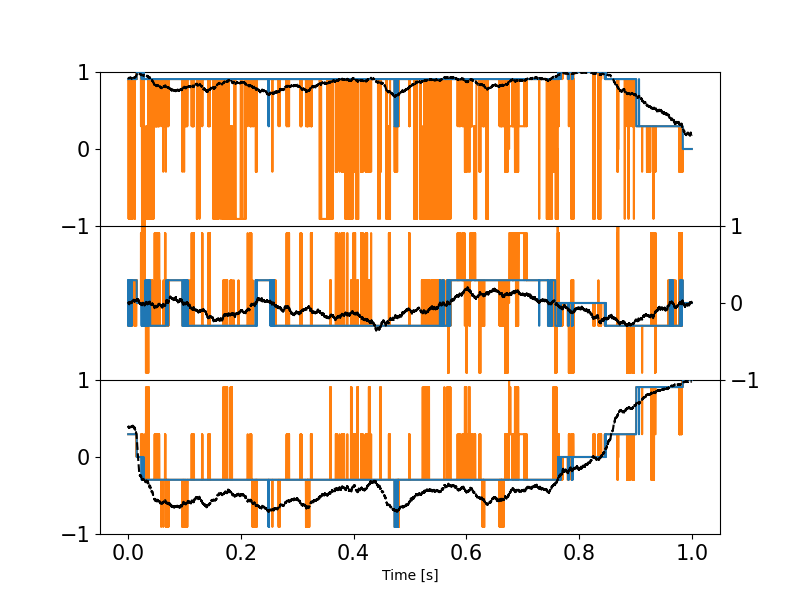
\includegraphics[width=\textwidth]{fig5.png}
	\caption{Model's estimation of dimer orientation over the simulation time, assuming uniform prior $p(\hat{\bf n}_\alpha)$, broken up into x, y, and z components for clarity. Blue line denotes the best result we can achieve (the reference orientation $\hat{\bf n}_{best}$ that is closest to the actual orientation), orange line denotes the result provided by eq~\ref{eq:bayes}: where the orange line is not visible, the model's prediction agrees with $\hat{\bf n}_{best}$. Dotted black line is the instantaneous orientation $\hat{\bf s}$.}
	\label{fig:uniform}
\end{figure} 

One reason we observe such large jumps in orientation estimated from scattering signals is that there is no simple correlation between the 'distance in scattering space' between scattering signals from two different orientations, and their separation in orientation space: even a large change in orientation can involve a small change in scattering. Combining this fact with use of a uniform prior, indicating essentially no knowledge of how orientation should behave, there is no constraint on how much estimated orientation can change from time-step to time-step. To improve the estimation we can therefore use knowledge of the physical limitations of the object in the trap and its dynamics, imposing a more physically grounded prior, accounting in this case for the fact that the motion of the dimer is limited due to the trap stiffness. Here the prior of the reference orientations $p(\hat{\bf n}_\alpha)$ was redefined at each time step as a Boltzmann distribution of the physical distance between the previous estimate $\hat{\bf n}_{est}(t-\Delta t)$ and each reference orientation $\hat{\bf n}_\alpha$. Put simply, we are reweighing our estimation based on the size of rotation required, with smaller movements being favoured over large movements:

\begin{align}
	p(\hat{\bf n}_\alpha)
	&=\frac{e^{\beta (\hat{\bf n}_\alpha 
			\cdot \hat{\bf n}_{est}(t-\Delta t))}}
	{\sum_{\alpha=1}^{n_{\rm ref}}
		e^{\beta (\hat{\bf n}_\alpha 
			\cdot \hat{\bf n}_{est}(t-\Delta t)}}
	\label{eq:boltz}
\end{align}
Here $\beta$ is a weighting factor describing the dimer's freedom of motion within the trap. As shown in Figure~\ref{fig:biased} implementation of Eq~\eqref{eq:boltz} helps significantly reduce the large random excursions of estimated orientation away from the 'best' result. 

\begin{figure}[h]
	\centering
	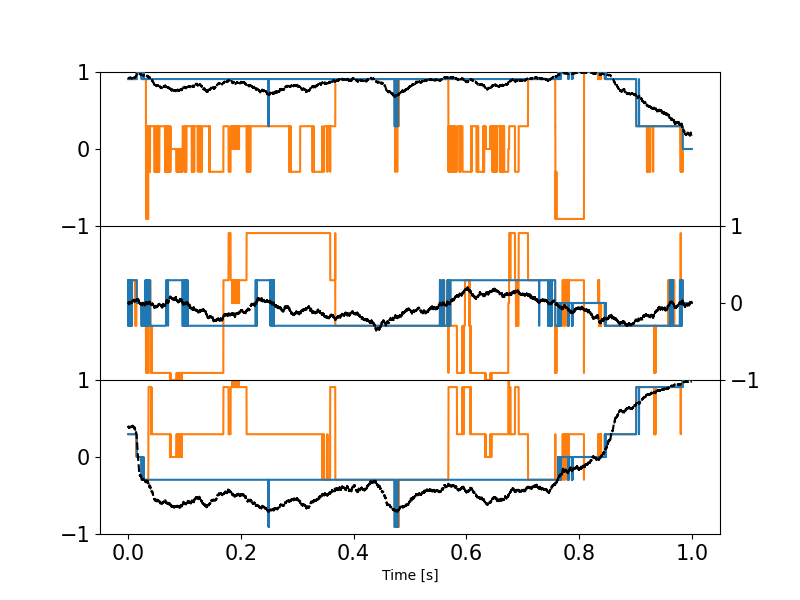
\includegraphics[width=\textwidth]{fig8a.png}
	\caption{\label{fig:biased}
		%
		Estimation of dimer orientation with $p(\hat{\bf n}_\alpha)$ defined
		by Eq~\eqref{eq:boltz}.  Blue line denotes the best result we can
		achieve, orange line denotes the result provided by eq~\ref{eq:bayes}.
		Dotted black line is the instantaneous orientation $\hat{\bf s}$ (see Section~\ref{sec:Bayes}).
		%
	}
\end{figure} 

The simulation data from Section~\ref{sec:brownian} was used to evaluate our model's performance --- covered in Section~\ref{sec:divergence}. By summing the divergence of each measurement across the entire simulation we get an evaluation of how well the model performed in estimating the dimer's orientation. To compare the effects of changing certain parameters on the performance of our model we compare our result of $K_{l,total}$ to a worst case scenario and evaluate how much it improves upon this, denoted as $F(K_l)$:
\begin{align}
	K_{l, \ total} &= \sum\limits_{\# =1}^{timesteps} K_{l,\#}
	\\
	K_{l, \ worst} &= \sum\limits_{\#=1}^{timesteps} \ln \left[\frac{1}{1/n_{ref}} \right]
	\\
	F(K_l) &= \frac{K_{l,\ worst}}{K_{l, \ total}}
\end{align}

The worst case scenario is akin to randomly choosing a reference
orientation at each time step. The greater the value of $F(K_l)$, the
better our model's confidence is in characterising the dimer's
motion. Because our model is dependent on several parameters we need
to a sophisticated method for understanding how these parameters
correlate with $F(K_l)$.

%%%%%%%%%%%%%%%%%%%%%%%%%%%%%%%%%%%%%%%%%%%%%%%%%%%%%%%%%%%%%%%%%%%%%
\subsection{Asymmetric dimer dynamics}
\label{sec:motion}
A simulation of a asymmetric dimer ($a_1=1\,\mu{\rm m}$, $a_2=0.5\,\mu{\rm m}$) 
trapped in an off-axis trapping orientation was used as a test case for our 
model, since it was previously shown that dimers can be optically rotated 

\begin{figure}[h!]
	\centering
	\begin{subfigure}{0.45\textwidth}
		\subcaption{}
		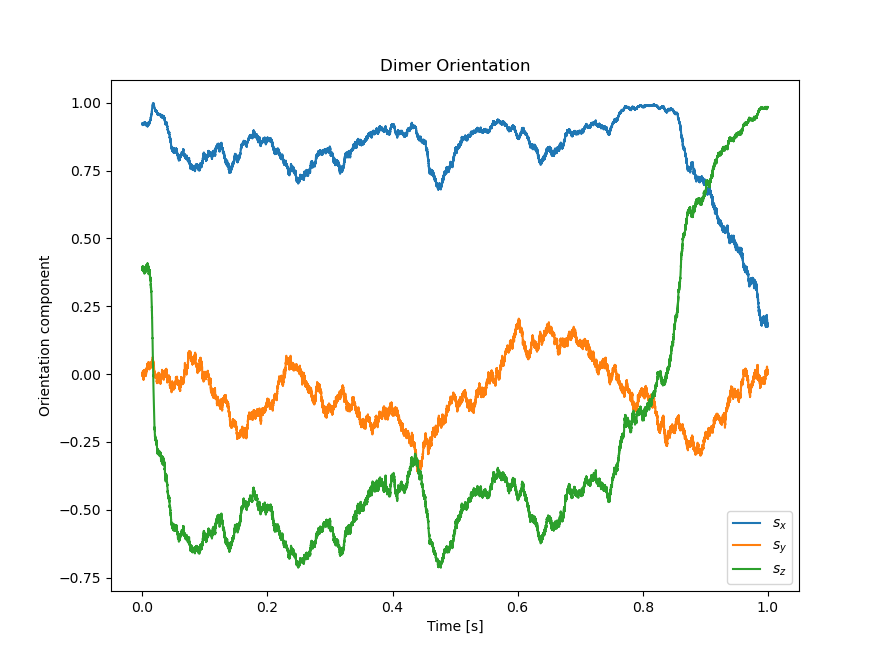
\includegraphics[width =\textwidth]{fig7a.png}
	\end{subfigure}
	\begin{subfigure}{0.45\textwidth}
		\subcaption{}
		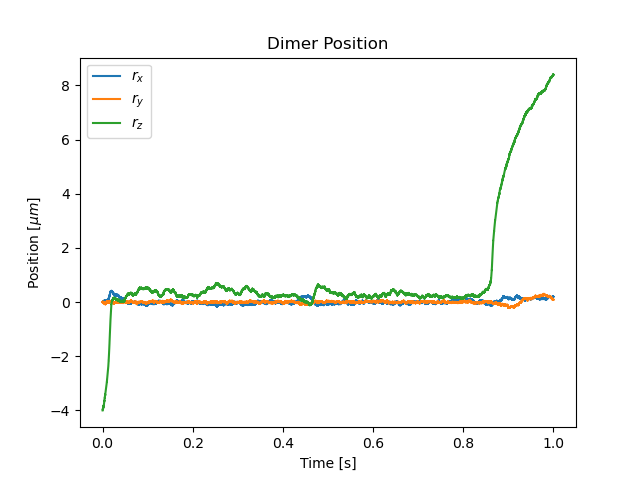
\includegraphics[width=\textwidth]{fig7b.png}
	\end{subfigure}
	\caption{Simulation results of: (a) the dimer's orientation vector with time, (b) the dimer's [x,y,z] position with time.}
	\label{fig:motion}
\end{figure}

In the simulations of Vigilante~\emph{et~al}.\ \cite{Vigilante2020Brownian_OT}, trapped symmetrical dimers were investigated; their findings showed that the optical torque on the dimer goes to zero while aligned vertically and is at its maximum in a horizontal alignment. However as seen in Figure~\ref{fig:motion} asymmetric dimers demonstrate dynamics that do not immediately achieve steady state. We chose to use asymmetric dimers as our benchmark due to this fact, as its orientational motion is far more complex than a symmetric dimer. In the future we hope to further investigate the motion of asymmetric dimers. 
%%%%%%%%%%%%%%%%%%%%%%%%%%%%%%%%%%%%%%%%%%%%%%%%%%%%%%%%%%%%%%%%%%%%%
%%%%%%%%%%%%%%%%%%%%%%%%%%%%%%%%%%%%%%%%%%%%%%%%%%%%%%%%%%%%%%%%%%%%%
\subsection{Accounting for sources of error in light scattering measurements}
When it comes to analysing light scattering from any size particle, error analysis becomes a significant factor. Typically this can be accounted for by averaging over long periods of time to get an assessment of the steady state conditions of the target particle. However in our case where we wish to know the instantaneous orientation, we instead have to rely on our understanding of how uncertainty can effect our model's performance. We identified two areas which are likely sources of error in our estimation: firstly, an incorrect modelling of the target particle, and secondly, signal noise arising from experimental factors. We highlight how we address these areas below. 
%%%%%%%%%%%%%%%%%%%%%%%%%%%%%%%%%%%%%%%%%%%%%%%%%%%%%%%%%%%%%%%%%%%%%
\subparagraph{Impact of incorrect dimer sizing}
\label{sec:lam}

One of the main limitations of our model is that we assume that the dimer being modelled in MSTM is accurate to the dimer being trapped in the optical tweezer. Sizing molecules accurately is a significant challenge for single particle analysis so there is bound to be some uncertainty with the measurements. We ran our model 3 times with the neural net being trained on a dimer of size ratio $1:1.95$, $1:2.00$ and $1:2.05$.
\begin{figure}[h!]
	\centering
	\begin{subfigure}{0.33\textwidth}
		\subcaption{}
		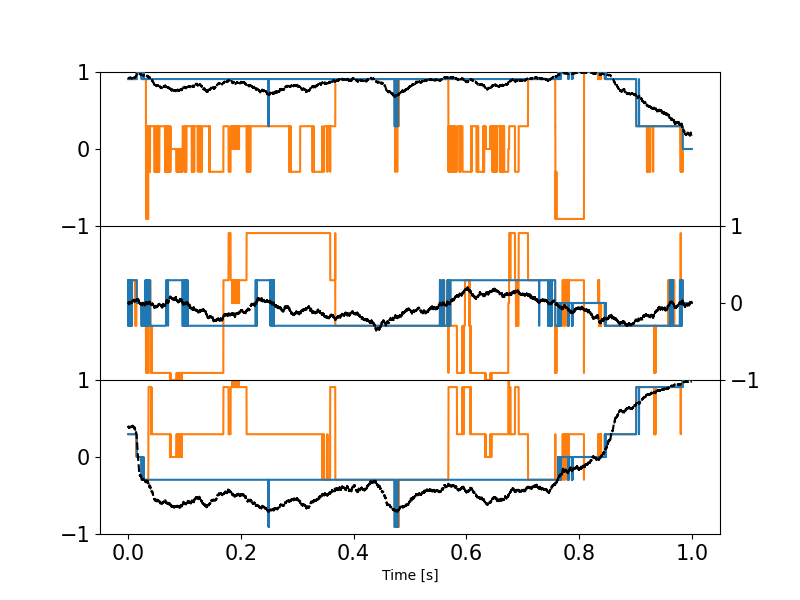
\includegraphics[width =\textwidth]{fig8a.png}
	\end{subfigure}
	\begin{subfigure}{0.31\textwidth}
		\subcaption{}
		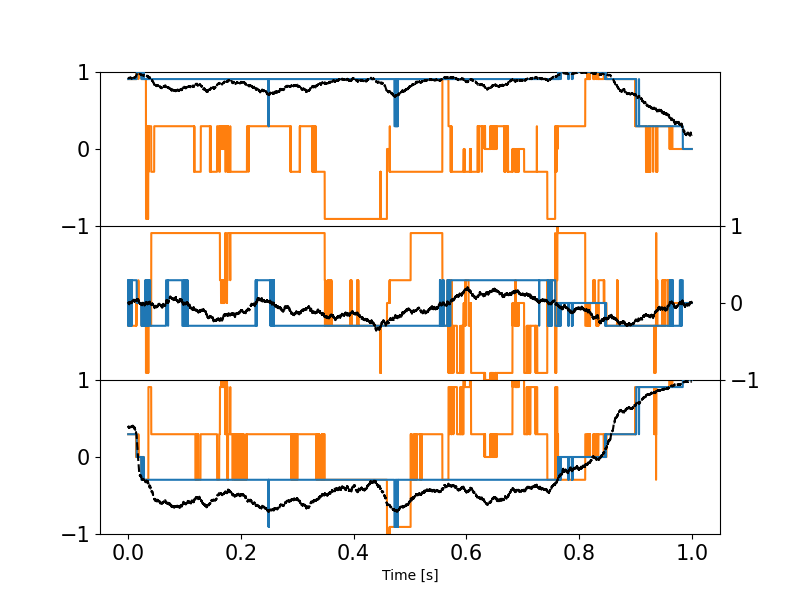
\includegraphics[width=\textwidth]{fig8b.png}
	\end{subfigure}
	\begin{subfigure}{0.31\textwidth}
		\subcaption{}
		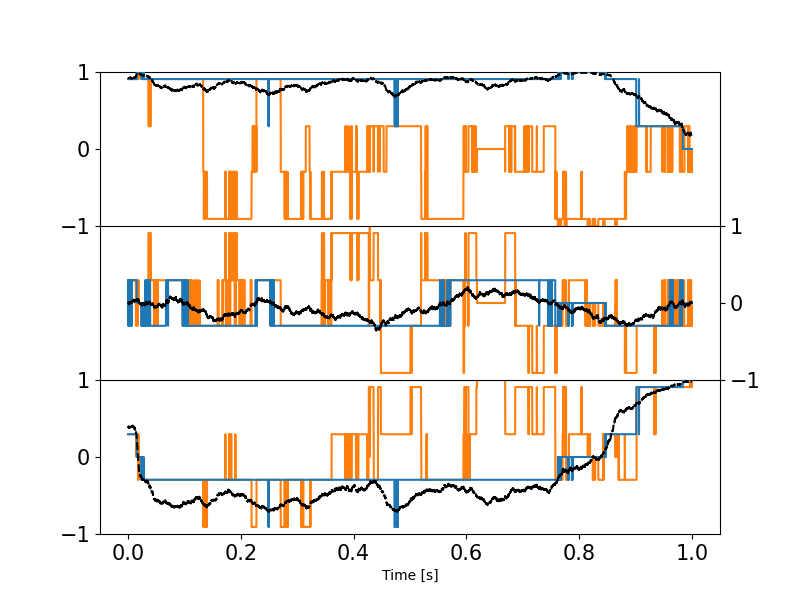
\includegraphics[width=\textwidth]{fig8c.png}
	\end{subfigure}
	\caption{Model estimates of orientation when neural net has been trained on dimer of size ratio: (a) 1:2 $[F(K_l)=9.456]$, (b) 1:2.05 $[F(K_l)=1.324]$, (c) 1:1.95 $[F(K_l)=1.325]$ ($n_{refs} = 30$)}
	\label{fig:size}
\end{figure}

As can be seen from Fig~\ref{fig:size}  even the slightest change in size ratio makes a very significant difference to the performance of our model. This amounts to just over $100 \ nm$ in the dimer's overall size, yet results in our model being correct from over 90 \% of the time to now as low as 30 \%. This highlights the importance of correctly sizing trapped entities before performing any in depth analysis of the scattering pattern, as even the slightest deviation can have a serious impact. We addressed this by increasing the number of available reference orientations from 30 to 126 (following the same procedure as given by \cite{Rey2006} to evenly space out the coordinates) and increasing the weighting factor in Eq~\ref{eq:boltz}. While this didn't have a significant improvement on the overall accuracy of the model, in the worst case having a slight increase from 30.5 \% to 40.3 \%, it did help to significantly reduce the magnitude between our model's estimations and the dimer's motion as seen below in Fig~\ref{fig:refs}.
\begin{figure}[h!]
	\centering
	\begin{subfigure}{0.31\textwidth}
		\subcaption{}
		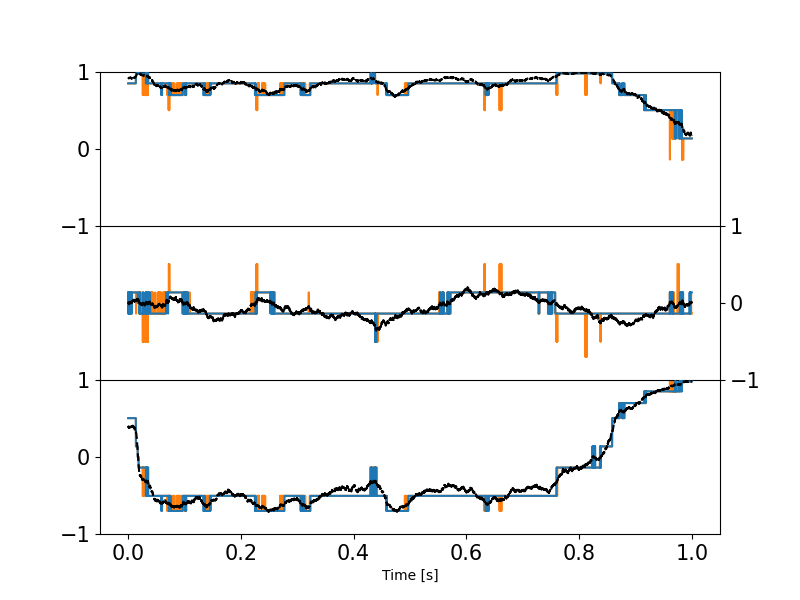
\includegraphics[width =\textwidth]{fig9a.png}
	\end{subfigure}
	\begin{subfigure}{0.31\textwidth}
		\subcaption{}
		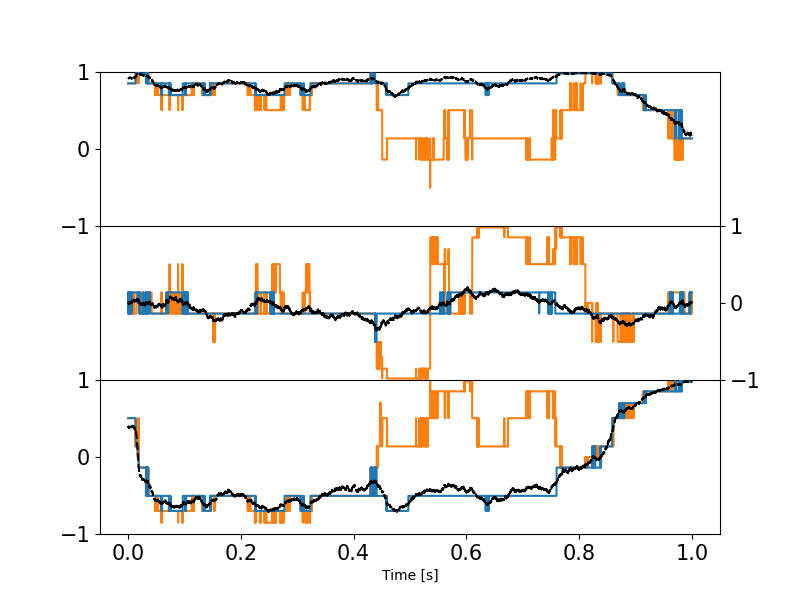
\includegraphics[width=\textwidth]{fig9b.png}
	\end{subfigure}
	\begin{subfigure}{0.31\textwidth}
		\subcaption{}
		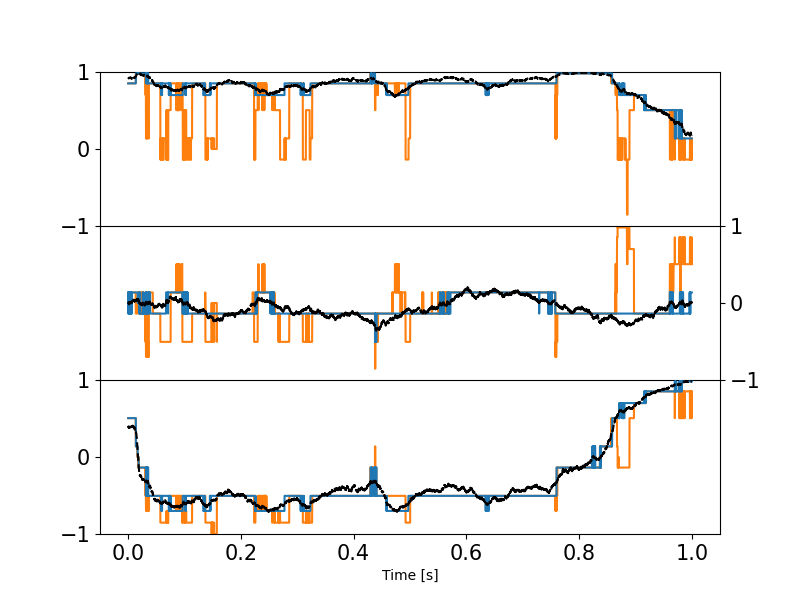
\includegraphics[width=\textwidth]{fig9c.png}
	\end{subfigure}
	\caption{Model estimates of orientation when neural net has been trained on dimer of size ratio: (a) 1:2 $[F(K_l)=11.756]$, (b) 1:2.05 $[F(K_l)=1.233]$, (c) 1:1.95 $[F(K_l)=2.128]$, ($n_{refs} = 126$)}
	\label{fig:refs}
\end{figure}

Notably the increasing the number of reference orientations had a greater effect when our neural network was trained on a 1:1.95 dimer than a 1:2.05 dimer. This suggests that overshooting our size estimate will be less detrimental to our estimation. Notably if the our sizing is off the neural network does not predict a smooth motion within the trap; instead predicting that the dimer is jumping back and forth between different orientations. This suggest that we can narrow down our estimate of the particle's size by assessing how the dimer is reorienting within the trap, as we should expect a smooth continuos prediction. Since we are working with a spherical dimer it also stands to reason that techniques such as image analysis could be used in part to address this, so long as the trapped entity is sufficiently illuminated. 
%%%%%%%%%%%%%%%%%%%%%%%%%%%%%%%%%%%%%%%%%%%%%%%%%%%%%%%%%%%%%%%%%%%%%
\subparagraph{Impact of measurement noise on model predictions}
\label{sec:epsilon}

So far a key assumption of the neural network implementation is that the detected scattering signal has no uncertainty associated with it. In reality of course scattering signals will always have some non-zero measurement noise. This can be attributed to a variety of factors, from a measurement bias in the detector, to the Brownian motion of the dimer itself. To explore the impact of measurement uncertainty on orientation estimation model performance we introduce a Gaussian noise to the measured signal:
\begin{align}
	I(\hat{\bf s}) = I(\hat{\bf s}) \pm \epsilon I(\hat{\bf s})
\end{align}
where $\epsilon$ is the percentage error associated with the scattering signal. Figure~\ref{fig:epsilon} shows the performance of the model at a range of $\epsilon$ using in-plane detector angles $15^{\circ}$, $55^{\circ}$, $90^{\circ}$ and out-of-plane detector at $75^{\circ}$, with $\beta$ set to $1$:

\begin{figure}[h!]
	\centering
	\begin{subfigure}{0.32\textwidth}
		\subcaption{}
		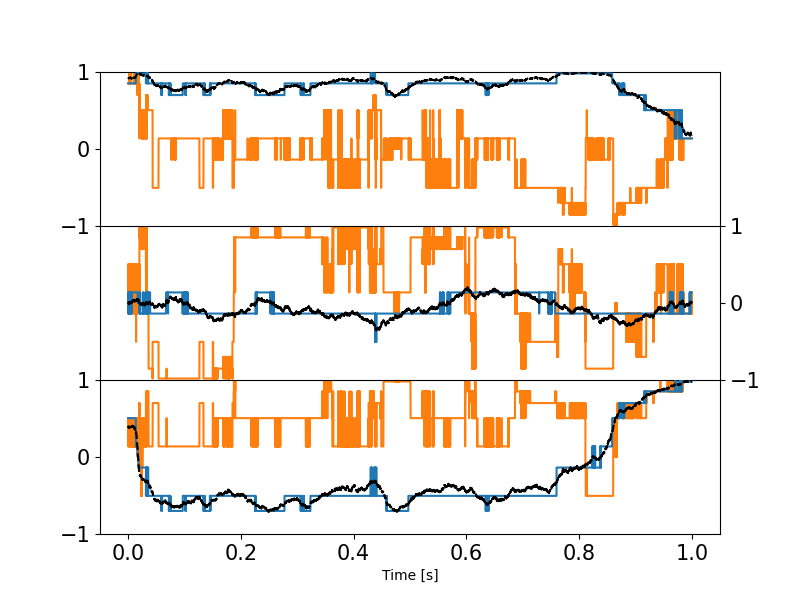
\includegraphics[width=\textwidth]{fig10a.png}
	\end{subfigure}
	\begin{subfigure}{0.32\textwidth}
		\subcaption{}
		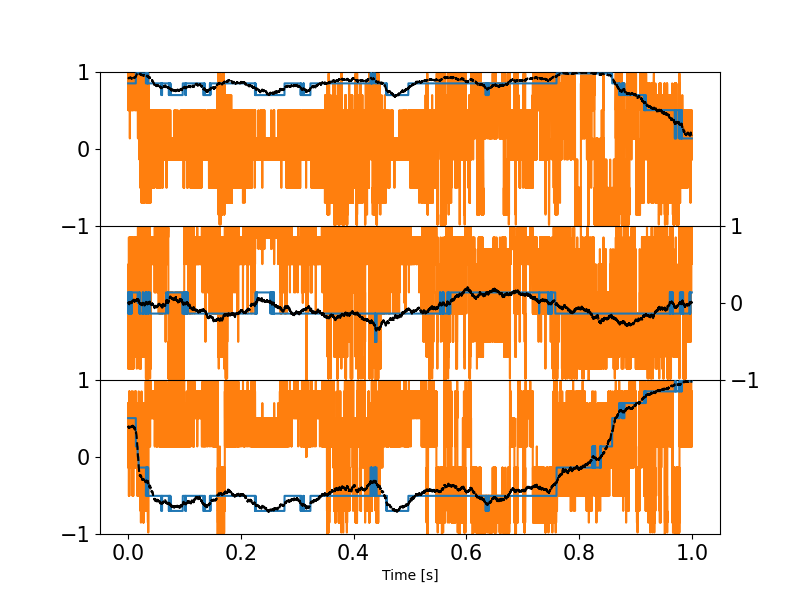
\includegraphics[width=\textwidth]{fig10b.png}
	\end{subfigure}
	\begin{subfigure}{0.32\textwidth}
		\subcaption{}
		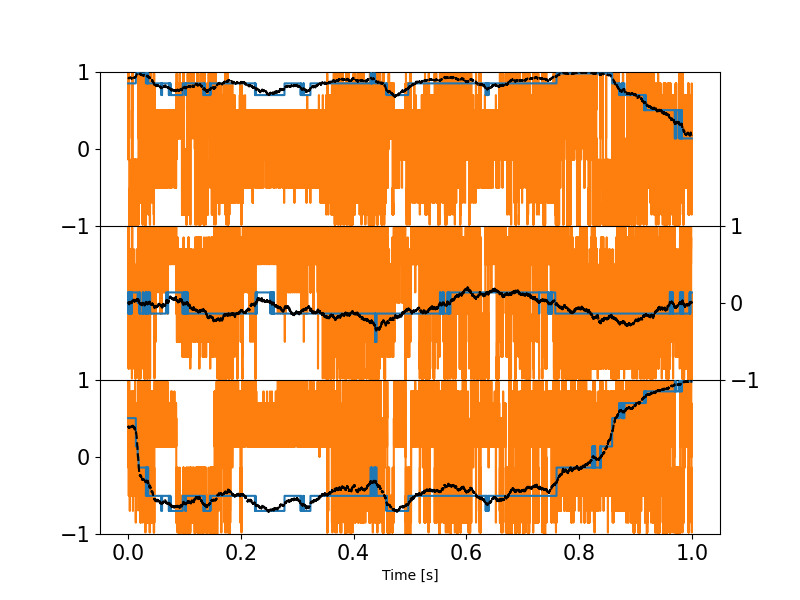
\includegraphics[width=\textwidth]{fig10c.png}
	\end{subfigure}
	\caption{Model prediction for signal error of (a) $1\%$ ~  $[F(K_l)=7.246]$, (b) $15\%$ $[F(K_l)=0.511]$, and (c) $25\%$ ~  $[F(K_l)=0.536]$.}
	\label{fig:epsilon}
\end{figure}

As can be seen from Figure~\ref{fig:epsilon}, the inclusion of signal noise quickly leads to a decrease in the model's performance. This is due to an inherent feature of the inverse scattering problem: two distinct regions in orientation space can become heavily intertwined and thus no longer well separated when mapped to intensity space (even though the mapping remains continuous): so even small uncertainties in the scattering data can lead to large 'mistakes' in the choice of orientation by the neural network. (Indeed if this was not the case the inverse scattering problem would be quite simple.) 

To reduce the effects of the signal noise we took the time average of the expected signal over $0.001 s$ and then had our neural network estimate the orientation based on the average signal.

\begin{figure}[h!]
	\centering
	\begin{subfigure}{0.32\textwidth}
		\subcaption{}
		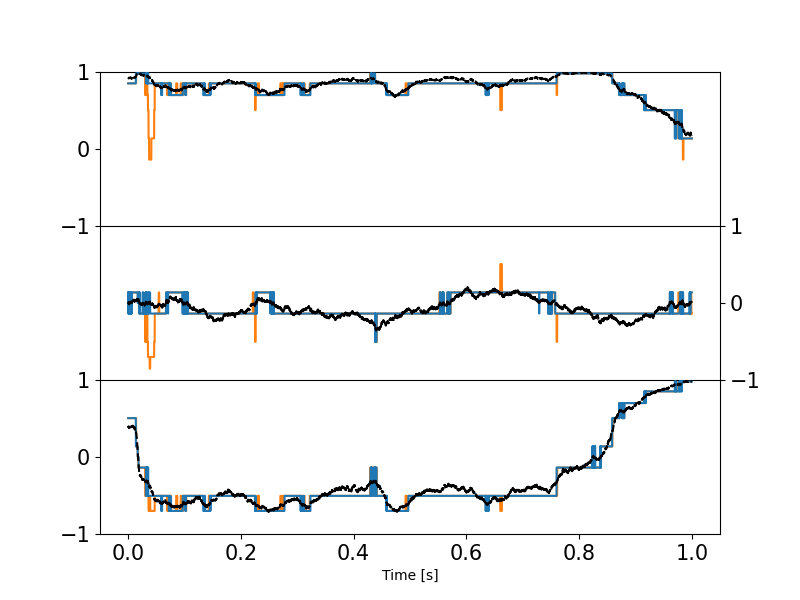
\includegraphics[width=\textwidth]{fig11a.png}
	\end{subfigure}
	\begin{subfigure}{0.32\textwidth}
		\subcaption{}
		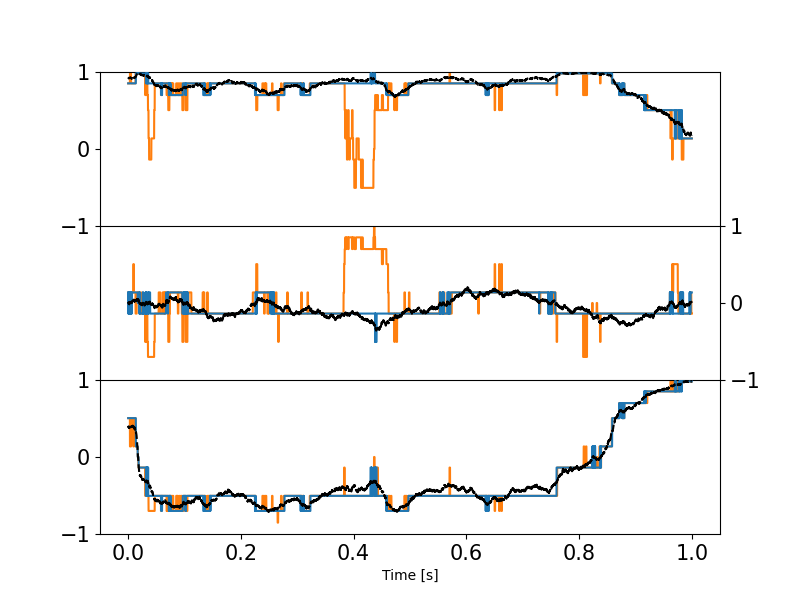
\includegraphics[width=\textwidth]{fig11b.png}
	\end{subfigure}
	\begin{subfigure}{0.32\textwidth}
		\subcaption{}
		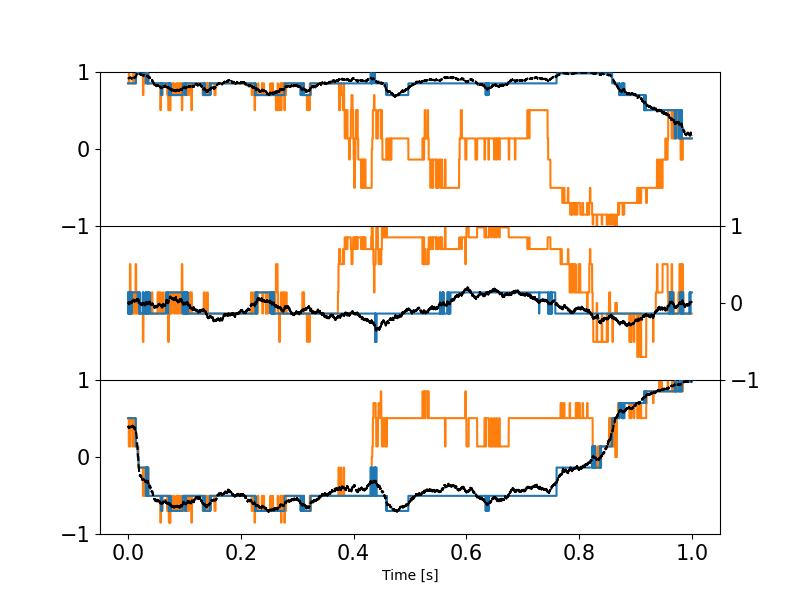
\includegraphics[width=\textwidth]{fig11c.png}
	\end{subfigure}
	\caption{Model prediction for signal error of (a) $1\%$ $[F(K_l)=4.823]$,  (b) $15\%$ $[F(K_l)=1.494]$, and (c) $25\%$ $[F(K_l)=0.882]$, time averaged over $1\,{\rm ms}$}
	\label{fig:time average}
\end{figure}
This resulted in a reduction in the overall signal noise and provided a higher degree of accuracy for our model. There appears to be no clear correlation between the length over which we time average and the performance of our model. Time averaging over every 0.05s resulted in a drastically worse performance; this is due to the fact that over longer time periods there is greater uncertainty regarding how the dimer's orientation has changed, thus tracking the instantaneous orientation becomes harder for the neural network. Fortunately, time averaging even over $1\,{\rm ms}$ seems to provide a satisfactory estimation of the dimer's angular dynamics within the optical trap.

From the above discussion it’s clear that estimation of the dimer’s orientation is a problem that can be endlessly tuned to fully maximise our end result. Here we simplify the problem somewhat by employing a relatively small finite number of 'reference orientations' to map between scattering and dimer orientation: the precision of estimation could be improved by utilising a greater number of reference orientations, although there remains a balance between the realisable precision of orientation estimate and the noise level of the scattering measurement. Another avenue to further explore would be using the method to optimise the choice of detection angles, essentially to find the region in the mapping between measured scattering and orientation that others the best degree of confidence through optimal separation of scattering signals for distinct orientations. For sequences of data such as dynamic measurements, a further potential enhancement would be to consider more complex correlations based on prior expectations of the dynamics. Here already we improve the method using a non-uniform prior based on only the immediately previous measurement in time (see Section 2.1): considering a non-uniform grouping of reference orientations might result in a better estimation, if we have information regarding the dimer’s preferred axis of rotation. 

%%%%%%%%%%%%%%%%%%%%%%%%%%%%%%%%%%%%%%%%%%%%%%%%%%%%%%%%%%%%%%%%%%%%%


\section{QPD Simulations}
A QPD is simply a measure of the total electric field incident on a photo diode, in order to accurately simulate a QPD response careful consideration of how the Electromagnetic fields are defined is required. 

\subsection{Incident beam}
\label{sec:fibre_scattering}
The incident beam is simple enough to define given our set up parameters, for the sake of simplicity we assume that our beam is a Laguerre-Gaussian beam of mode $[0.0, 0.0]$ (which is simply a pure Gaussian beam). *Ott* uses a point matching approach to approximate the beam shape coefficients of the incident field by fitting it to the far field estimate, the beam is of the form:

\begin{align}
	E_{inc}(kr)=\sum^\infty_n\sum^n_{m=-n}a_{mn}RgM_{nm}(kr)+b_{nm}RgN_{nm}(kr)
\end{align}

Where $RgM_{nm}(kr)$ \& $RgN_{nm}(kr)$ are regular vector spherical wave functions, *ott* allows us to change the basis of the the incident beam to suit our needs, because we are measuring in the far field we want to set our incident beam to be an outgoing spherical wave so that we can compute the intensity on the QPD. For spherical waves the field can either be expressed as an incoming/outgoing wave (with a singularity at the origin) or as a regular wave around the origin; for incoming/outgoing waves the wave functions use the first/second forms of the Hankel function respectfully. In order to compute the regular spherical wave at the origin we replace the Hankel function with the Bessel function which is simply the average of the first and second forms of the Hankel function, so at the origin we avoid a singularity of the EM field.  

We can if we want further restrict the incident beam by applying setting the truncation angle to match our microscope object, this essentially applies a cut off point to the In order to compute the scattering from the target particle *ott* uses the t-matrix method, this is not essential for a simple sphere but is far more important for complex shaped particles such as our dimers. If the T-matrix is loaded in from *mstm* we need to convert the *mstm* t-matrix to a form more suitable for *ott*:

\begin{align}
	\begin{pmatrix}
		p_{nm}\\
		q_{nm}
	\end{pmatrix} =T 
	\begin{pmatrix}
		a_{nm}\\
		b_{nm}
	\end{pmatrix} = 
	\begin{pmatrix}
		aT^{TM}_{nm} & aT^{TE}_{nm}\\ 
		bT^{TM}_{nm} & bT^{TE}_{nm}
	\end{pmatrix}
	\begin{pmatrix}
		a_{nm}\\
		b_{nm}
	\end{pmatrix}
\end{align} 

For *mstm* the T-matrix is packed as a column vector:

\begin{align}
	T_{MSTM} = 
	\begin{bmatrix} 
		aT^{TE}_{n,-n} & bT^{TE}_{n,-n} \\ 
		aT^{TE}_{n, -n+1} & bT^{TE}_{n, -n+1} \\ 
		... & ...\\ 
		aT^{TE}_{n,n} & bT^{TE}_{n,n} \\ 
		----&----\\ 
		bT^{TM}_{n,-n} &bT^{TM}_{n,-n} 
	\end{bmatrix}
\end{align}

Where as *ott* packs packs the T-matrix with sub matrices:

\begin{align}
	T_{Ott} = 
	\begin{bmatrix} 
		\begin{pmatrix}
			aT^{TM}_{n,-n} & aT^{TE}_{n,-n}\\ 
			bT^{TM}_{n,-n}&bT^{TE}_{n,-n}
		\end{pmatrix} \\ 
		\begin{pmatrix}
			aT^{TM}_{n,-n+1} & aT^{TE}_{n,-n+1}\\ 
			bT^{TM}_{n,-n+1} & bT^{TE}_{n,-n+1}
		\end{pmatrix}\\
		....\\ 
		\begin{pmatrix}
			aT^{TM}_{nm} & aT^{TE}_{nm}\\ 
			bT^{TM}_{nm} & bT^{TE}_{nm}
		\end{pmatrix}
	\end{bmatrix}
\end{align}

\subsection{Scattered and Total Fields}
With the T-matrix in hand we can compute the scattered beam by multiplying our beam shape coefficients with the T-matrix to get out the scattered field. Now in order to simulate a real QPD we need to account for the motion of our target particle within the trap, taking a typical trajectory file we read off each line in order to translate and rotate the beam. Translation is a rather simple process, simply involving us to shift the beam laterally, small deflections are generally unnoticeable for the incident beam but are much more noticeable in the scattered field (the below figure shows the result of shifting the incident beam $1\mu m$ to the right):

The QPD does not just pick up the scattered light however, it instead is receiving a combined signal from both the incident field and scattered field simultaneously, as mentioned by \textcolor{red}{Rohrbach} the total intensity can be computed by taking the magnitude of both the incident field *focused at the origin $[0,0,0]$* and the scattered field originating from $[\delta x, \delta y, \delta z]$ (top left and bottom right plots in the above figure). This means we do not need to worry about any translation effects being 'double-counted' in the QPD's signal as we are only shifting the scattered field meaning the QPD signal is only picking up the interference due to the shifted scattered field. I conducted some unitary tests where I scanned the beam position laterally along the x-axis and measured the QPD's 'x-signal' for x, circular and y-polarized light which yielded the following QPD responses. The target particle was $1.57\ \mu m$ and the scan range is set to $[-4, 4 \mu m]$

Where $S_x$ is given in blue, and $S_y$ is given in orange, the plots make it clear that the polarisation of the beam have a minimal effect on the QPD signals if the particle is traversing in one direction, its clear that the displacement from the beam centre is far more important than the polarization of said beam. This is backed up when we look at \textcolor{red}{Rohrbach's} results, who studied a $150\ nm$ sphere ($n=1.57$) submerged in water with a focusing lens of numerical aperture 1.2, and beam power of $3\ mW$. The condensing lens' numerical aperture was not set to a particular value and was instead varied between 0.13-1.2, as a compromise we selected a condenser numerical aperture of 0.525, corresponding to a acceptance angle of $31.6^\circ$. 

Where the points are Rohrbach's results and the solid line's are our QPD's own replication. The dashed horizontal lines on the left represent the maximum displacement in the lateral displacement which is given by the combined beam radius and particle radius (assuming a beam radius of $0.54\ \mu m$); we can say that any displacements beyond this distance, while non-zero these displacements are unlikely to occur while a particle is trapped at the focus. Whereas the right most plot's dashed horizontal lines represents the Rayleigh range of the Gaussian beam, this represents the transition between plane wave and spherical wave regimes. Interestingly while our results close to Rohrbach's while close to the focus we see it begins to diverge beyond the first peak, this shouldn't be an issue for a typical optical tweezer calibration as we can assume that the maximum displacement will be within this linear regime. 

Now the above plots only consider the QPD response to movements along the cartesian axis, however obviously for any Brownian motion the movements are a combination of displacements in each cartesian direction. We might assume naively that any displacement $\Delta r$ will result in a linear combination of QPD responses; for low precision force measurements this assumption is adequate, however when high precision is required we find that this assumption is longer adequate due to something referred to as cross-talk. Cross talk arises when movement in one direction results in a QPD response change in the other orthogonal direction, there is no one reason for this effect, it could be a result of differing sensitivity in the photo diodes, it could be because the scattering is slightly asymmetric meaning the scattering falls outside the QPD, or it could be a result of mis-alignment in the set up. This can have unintended effects, for example it may lead to the apparent rise of a curved trajectory rather than a straight path: Consider a particle moving purely along the x-axis, with 0 cross-talk the QPD response should perfectly match the above curve $S_x(x,0,z_0)$, with $S_y$ being flat in comparison; if however there is cross talk between the channels then $S_y$ will have some significant non-zero value (or it may even grow with increasing displacement), implying that the particle is actually moving in both the x and y directions simultaneously.  First we checked for this by measuring the QPD response for random positions within the XY plane:

Where $S_x$ is plotted on top and $S_y$ is plotted below, as shown by the above plot we see that they still possess similar shapes to the previous plots but now with additional noise terms, making it clear that for any trajectory there will be cross talk. This means that trying to get a one-to-one measurement of the particle's displacement is not possible by simply looking at the QPD response, to do that we can need to calibrate the trap. 

\textcolor{red}{Berg and Flyvbjerg} have an excellent breakdown for accurately calibrating an optical tweezer, in addition they discuss how to minimise cross-talk effects. For two correlated power spectra, the cross correlation is given as:

\begin{align}
	P_{x} = |\hat{S}_x(f)|^2 \\ 
	P_{y} = |\hat{S}_y(f)|^2 \\
	\rightarrow P_{xy} = Re(\hat{S}_x\hat{S}^*_y)
\end{align}

Now if the two directions are correlated then $|P_{xy}|^2/P_xP_y$  should be non-zero for all frequencies, in order to eliminate cross-talk effects we need to minimise the cross-correlation for all frequencies. They showed that it is possible to find a transformation of the time series $(x(t), y(t))$  to one that possesses the property that $P_{x'y'}(f)=0$ for all frequencies. They found these transformed positions by minimising the sum cross-correlation:

\begin{align}
	\sum\frac{P_{x'y'}}{P_{x'}P_{y'}} = \sum\frac{(1+bc)P_{xy}+cP_x+bP_y}{(P_x+2bP_{xy}+b^2P_y)(Py+2cP_{xy}+c^2P_y)}
\end{align}

Where b and c are fitting parameters, by minimising this function one can adjust each spectra in order to eliminate cross talk effects and provide a more accurate calibration of the optical trap. Furthermore with the fitting completed, the time series can be then transformed in order to eliminate the cross talk effects:

\begin{align}
	x'(t) = S_x(t) + bS_y(t),\ y'(t) = S_y(t) + cS_x(t)
\end{align}

Where $x'$ and $y'$ are now uncoupled coordinates that when Fourier transformed provide the uncorrelated power spectrum. With the fitting complete we can now adjust our time series in order to get a replication of the lateral trajectory. 

\section{Rotations and Asymmetric particles}
Rotational motion is something that is not often necessarily considered when characterising Brownian motion, often because separating the contributions from rotational and translational motion is challenging. Depending on the rotational and translational trap stiffness the collected QPD signal will be aliased and typical calibration techniques cannot characterise the particle and trap interactions. This is often why most of the research into trapping asymmetric objects does not delve into power spectra analysis, as there is no real way of modelling the QPD response from an asymmetric object. 

Now for isotropic scatterers any rotation is often not an issue when it comes to QPD analysis, even if a sphere rotates $180^{\circ}$the scattering should be identical (assuming its relative position is the same). Now *ott* deals with both translations and rotations by moving the beam itself and computing the scattering from by once again expanding the spherical wave functions, the problem that arises from this is that the portion of the spherical wave that is evaluated by the QPD will pick up said rotation and produce a non-zero signal even if the scatterer in question is isotropic. This means we need to counter rotate the total field prior to collecting the QPD signal, this captures the effects of an anisotropic scatterer but has no effect for an isotropic scatterer. As a test the QPD response from an isotropic sphere of $1.57 \ \mu m$ was collected at multiple angles, between 0 and $2\pi$, then as a comparison a symmetrical and 1:2 dimer were also subjected to the same rotations and their QPD responses evaluated. 

Where on the left we have an isotropic sphere, then a symmetrical dimer, and lastly a 1:2 dimer. The left most plot shows that simply using the inverted rotation matrix is sufficient to prevent rotation effects being double counted.
For dimers however, rotating about a given axis gives us a clear change in the signal for even a slight rotation about any axis. 

\section{Power Spectra of single sphere vs spherical aggregates}
In order to verify that the QPD is outputting correct signals we first compared the module to the only other known instance of simulating a QPD response, that being the work of \textcolor{red}{Rorhbach}. In their paper they looked at the signal response produced by a single sphere ($r = 150\ nm$, $n = 1.57$) being scanned along the three Cartesian axis in the proximity 
of a $1064\ nm$ NIR beam with a numerical aperture of 1.2. As shown by fig~\ref{fig:Rohrbach} the two responses are remarkably accurate close to the origin; with only slight deviations as you move past the harmonic region, the difference can be explained due to how the two evaluate the total fields. Where in our case the incident and scattered fields are reduced to 0 at the origin, whereas Rohrbach's work evaluates the fields the fields as being non-zero at all points, as you move beyond the origin this discrepancy grows. 

Since we are only interested in the dynamics of spherical aggregates upon reaching equilibrium we do not need to be concerned about the deviation from Rohrbach's results so long as the particle's displacement does not exceed the linear region at the origin. The axial response curve is slightly more involved, requiring that the condenser lens numerical aperture is adjusted until a harmonic response curve is achieved \cite{Friedrich2012}. 

In order to verify that the QPD can accurately capture the dynamics of the target particle we first simulated a single sphere ($a = 1\mu\ m$, $n=1.59$) in the focus of a $1064\ nm$ laser. Using \textit{ott} the trap stiffness is computed by applying a linear fit to the force-displacement curve along the x and y axis'; for a linearly polarised trap the gradient force is greater in the polarisation direction than transverse case. We see this reflected in the simulated QPD, the fitted Lorentzian curves have different corner frequencies indicating that the beam's polarisation is influencing the dynamics of the trap. 

Next we consider a dimer composed of two sphere's similar to the previous sphere, we again apply the QPD module to reproduce the power spectrum. Previous experimental work found that a pair of trapped beads would half the corner frequency from the reported power spectra. However, in our own simulations we see instead an increase in the expected trapping force from our QPD method, with the maximum trap stiffness expected for a dimer of size ratio 5. Compared to \textit{ott} in which the maximum trapping strength is expected at a size ratio of 2. This can be somewhat explained by the fact that as the second sphere shrinks the centre of diffusion approaches the centre of the larger sphere and thus the dimer's orientational behaviour is similar to a single sphere, only subject to slight Brownian motion. Therefore one should expect that for aggregates containing multiple sized particles (e.g. cellular samples) typical characterisation techniques may over estimate the strength of the trap.


%%%%%%%%%%%%%%%%%%%%%%%%%%%%%%%%%%%%%%%%%%%%%%%%%%%%%%%%%%%%%%%%%%%%%
\section{Conclusion}
\label{sec:Conclusion}

We have developed a method for measuring the dynamics of an optically-trapped colloidal objects based purely on measurements of the object's light scattering at a small number of detection angles. We demonstrate the method using the orientation of an asymmetric dimer as the dynamic variable and object of interest respectively, but in principle the model can be applied to any characteristic that impacts the light scattering pattern produced by a trapped entity such as size and shape. The MSTM package is a flexible tool for calculating the light scattering of complex objects using a representation of the object as a set of micro-particles, enabling training of a neural network to enable categorisation of the mapping between scattering and trapped object characteristics. By taking account of the physically realistic behaviour of the trapped object and the characteristics of the trap (which impact the dynamics of the object), the Bayesian inference method can be re ned to provide a reliable estimation of object characteristics of interest, even in the presence of measurement noise. Fundamentally, the inverse scattering problem is difficult to solve, since the mapping between object characteristics and scattering can be highly complex. We determined the minimum number of detectors required for a reliable estimation in the presence of measurement noise; furthermore, we demonstrated that the arrangement of these detectors is critical for a reliable estimation of an objects orientation. However, Bayesian inference based on neural network estimation of the mapping provides a powerful method for practical applications, extending the use of optical trapping beyond measuring microscopic force response toward detailed structural and dynamic information about complex trapped entities. 
